
\chapter{Calculus}

Mathematics is the investigation of an artificial world: a universe populated by abstract entities and rigid rules governing those entities.  Mathematicians devoted to the study and advancement of pure mathematics have an extremely well-developed respect for these rules, for the integrity of this artificial world depends on them.  In order to preserve the integrity of their artificial world, their collective work must be \textit{rigorous}, never allowing for sloppy handling of the rules or allowing intuitive leaps to be left unproven.

However, many of the tools and techniques developed by mathematicians for their artificial world happen to be extremely useful for understanding the real world in which we live and work, and therein lies a problem.  In applying mathematical rules to the study of real-world phenomena, we often take a far more pragmatic approach than any mathematician would feel comfortable with.

The tension between pure mathematicians and those who apply math to real-world problems is not unlike the tension between linguists and those who use language in everyday life.  All human languages have rules (though none as rigid as in mathematics!), and linguists are the guardians of those rules, but the vast majority of human beings play fast and loose with the rules as they use language to describe and understand the world around them.  Whether or not this ``sloppy'' adherence to rules is good depends on which camp you are in.  To the purist, it is offensive; to the pragmatist, it is convenient.

I like to tell my students that mathematics is very much like a language.  The more you understand mathematics, the larger ``vocabulary'' you will possess to describe principles and phenomena you encounter in the world around you.  Proficiency in mathematics also empowers you to grasp relationships between different things, which is a powerful tool in learning new concepts.

This book is not written for (or by!) mathematicians.  Rather, it is written for people wishing to make sense of industrial process measurement and control.  This chapter of the book is devoted to a very pragmatic coverage of certain mathematical concepts, for the express purpose of applying these concepts to real-world systems. 

\vskip 10pt

Mathematicians, cover your eyes for the rest of this chapter!



% \filbreak
% \section{Algebraic identities and laws}





% \filbreak
% \section{Trigonometric identities and laws}





% \filbreak
% \section{Vectors}





\filbreak
\section{Introduction to calculus}

Few areas of mathematics are as powerfully useful in describing and analyzing the physical world as calculus: the mathematical study of \textit{changes}.  Calculus also happens to be tremendously confusing to most students first encountering it.  A great deal of this confusion stems from mathematicians' insistence on rigor\footnote{In mathematics, the term \textit{rigor} refers to a meticulous attention to detail and insistence that each and every step within a chain of mathematical reasoning be thoroughly justified by deductive logic, not intuition or analogy.} and denial of intuition.  

Look around you right now.  Do you see any mathematicians?  If not, good -- you can proceed in safety.  If so, find another location to begin reading the rest of this chapter.  I will frequently appeal to practical example and intuition in describing the basic principles of single-variable calculus, for the purpose of expanding your mathematical ``vocabulary'' to be able to describe and better understand phenomena of change related to instrumentation.

Silvanus P. Thompson, in his wonderful book \textit{Calculus Made Simple} originally published in 1910, began his text with a short chapter entitled, ``To Deliver You From The Preliminary Terrors\footnote{The book's subtitle happens to be, \textit{Being a very-simplest introduction to those beautiful methods of reckoning which are generally called by the terrifying names of the differential calculus and the integral calculus}.  Not only did Thompson recognize the anti-pragmatic tone with which calculus is too often taught, but he also infused no small amount of humor in his work.}.''  I will follow his lead by similarly introducing you to some of the notations frequently used in calculus, along with very simple (though not mathematically rigorous) definitions.

\vskip 10pt

When we wish to speak of a change in some variable's value (let's say $x$), it is common to precede the variable with the capital Greek letter ``delta'' as such:

$$\Delta x = \hbox{``Change in } x \hbox{''}$$

An alternative interpretation of the ``delta'' symbol ($\Delta$) is to think of it as denoting a \textit{difference} between two values of the same variable.  Thus, $\Delta x$ could be taken to mean ``the difference between two values of $x$''.  The cause of this difference is not important right now: it may be the difference between the value of $x$ at one point in time versus another point in time, it may be the difference between the value of $x$ at one point in space versus another point in space, or it may simply be the difference between values of $x$ as it relates to some other variable (e.g. $y$) in a mathematical function.  If we have some variable such as $x$ that is known to change value relative to some other variable (e.g. time, space, $y$), it is nice to be able to express that change using precise mathematical symbols, and this is what the ``delta'' symbol does for us.

\filbreak

For example, if the temperature of a furnace ($T$) increases over time, we might wish to describe that change in temperature as $\Delta T$:

$$\includegraphics{calculus_01.eps}$$

The value of $\Delta T$ is nothing more than the difference (subtraction) between the recent temperature and the older temperature.  A rising temperature over time thus yields a positive value for $\Delta T$, while a falling temperature over time yields a negative value for $\Delta T$.

We could also describe differences between the temperature of two \textit{locations} (rather than a difference of temperature between two \textit{times}) by the notation $\Delta T$, such as this example of heat transfer through a heat-conducting wall where one side of the wall is hotter than the other:

$$\includegraphics{calculus_02.eps}$$

Once again, $\Delta T$ is calculated by subtracting one temperature from another.  Here, the sign (positive or negative) of $\Delta T$ denotes the \textit{direction} of heat flow through the thickness of the wall.

\vskip 10pt

One of the major concerns of calculus is changes or differences between variable values lying \textit{very close to each other}.  In the context of a heating furnace, this could mean increases in temperature over miniscule time periods.  In the context of heat flowing through a wall, this could mean differences in temperature sampled between points within the wall immediately adjacent each other.  If our desire is to express the change in a variable between neighboring points along a continuum rather than over some discrete period, we may use a different notation than the capital Greek letter delta ($\Delta$); instead, we use a lower-case Roman letter $d$ (or in some cases, the lower-case Greek letter delta: $\delta$).

Thus, a change in furnace temperature from one instant in time to the next could be expressed as $dT$ (or $\delta T$), and likewise a difference in temperature between two adjacent positions within the heat-conducting wall could also be expressed as $dT$ (or $\delta T$).  Just as with the ``delta'' ($\Delta$) symbol, the changes references by either $d$ or $\delta$ may occur over a variety of different domains.  

We even have a unique name for this concept of extremely small differences: whereas $\Delta T$ is called a \textit{difference} in temperature, $dT$ is called a \textit{differential} of temperature.  The concept of a differential may seem redundant to you right now, but they are actually quite powerful for describing \textit{continuous changes}, especially when one differential is related to another differential by ratio (something we call a \textit{derivative}).   \index{Differential, calculus}  \index{Derivative, calculus}  

\vskip 10pt

Another major concern in calculus is how quantities accumulate, especially how differential quantities add up to form a larger whole.  A furnace's temperature rise since start-up ($\Delta T_{total}$), for example, could be expressed as the accumulation (sum) of many temperature differences ($\Delta T$) measured periodically.  The total furnace temperature rise calculated from a sampling of temperature once every minute from 9:45 to 10:32 AM could be written as:

$$\Delta T_{total} = \Delta T_{9:45} + \Delta T_{9:46} + \cdots \Delta T_{10:32} = \hbox{Total temperature rise over time, from 9:45 to 10:32}$$

A more sophisticated expression of this series uses the capital Greek letter sigma (meaning ``sum of'' in mathematics) with notations specifying which temperature differences to sum:

$$\Delta T_{total} = \sum_{n=9:45}^{10:32} \Delta T_n = \hbox{Total temperature rise over time, from 9:45 to 10:32}$$

However, if our furnace temperature monitor scans at an infinite pace, measuring temperature \textit{differentials} ($dT$) and summing them in rapid succession, we may express the same accumulated temperature rise as an \textit{infinite} sum of \textit{infinitesimal} (infinitely small) changes, rather than as a finite sum of temperature changes measured once every minute.  Just as we introduced a unique mathematical symbol to represent differentials ($d$) over a continuum instead of differences ($\Delta$) over discrete periods, we will introduce a unique mathematical symbol to represent the summation of differentials ($\int$) instead of the summation of differences ($\sum$):

$$\Delta T_{total} = \int_{9:45}^{10:32} dT = \hbox{Total temperature rise over time, from 9:45 to 10:32}$$

This summation of infinitesimal quantities is called \textit{integration}, and the elongated ``S'' symbol ($\int$) is the \textit{integral} symbol.  \index{Integral, calculus}

\vskip 10pt

These are the two major ideas and notations of calculus: \textit{differentials} (tiny changes represented by $d$ or $\delta$) and \textit{integrals} (accumulations represented by $\int$).  Now that wasn't so frightening, was it?













\filbreak
\section{The concept of differentiation}

Suppose we wished to measure the rate of propane gas flow through a hose to a torch:

$$\includegraphics{calculus_03.eps}$$

Flowmeters appropriate for measuring low flow rates of any gas are typically very expensive, making it impractical to directly measure the flow rate of propane fuel gas consumed by this torch at any given moment.  We could, however, \textit{indirectly} measure the flow rate of propane by placing the tank on a scale where its mass ($m$) could be monitored over time.  By taking measurements of mass over short time periods ($\Delta t$), we could calculate the corresponding differences in mass ($\Delta m$), then calculate the ratio of mass lost over time to calculate average mass flow rate ($\overline{W}$):

$$\overline{W} = {\Delta m \over \Delta t} = \hbox{Average mass flow rate}$$ 

\noindent
Where,

$\overline{W}$ = Average mass flow rate within each time period (kilograms per minute)

$\Delta m$ = Measured mass difference over time period (kilograms)

$\Delta t$ = Time period of mass measurement sample (minutes)

\vskip 10pt

Note that flow rate is a ratio (quotient) of mass change over time change.  The units used to express flow even reflect this process of division: kilograms \textit{per} minute.

$$\overline{W} = {\hbox{[kg]} \over \hbox{[min]}} = \hbox{Average mass flow rate} = \left[{\hbox{kg} \over \hbox{min}}\right]$$ 

\filbreak

Graphed as a function over time, the tank's mass will be seen to decrease as time elapses.  Each dot represents a mass and time measurement coordinate pair (e.g. 20 kilograms at 7:38, 18.6 kilograms at 7:51, etc.):

$$\includegraphics{calculus_04.eps}$$

We should recall from basic geometry that the slope of a line or line segment is defined as its \textit{rise} (vertical height) divided by its \textit{run} (horizontal width).  Thus, the average mass flow rate calculated within each time period may be represented as the pitch (slope) of the line segments connecting dots, since mass flow rate is defined as a change in mass per (divided by) change in time.

Periods of high propane flow (large flame from the torch) show up on the graph as steeply-pitched line segments.  Periods of no propane flow reveal themselves as flat portions on the graph (no rise or fall over time).

\vskip 10pt

If the determination of average flow rates between significant gaps in time is good enough for our application, we need not do anything more.  However, if we wish to detect mass flow rate at any particular \textit{instant} in time, we need to perform the same measurements of mass loss, time elapse, and division of the two at an infinitely fast rate.

\filbreak

Supposing such a thing were possible, what we would end up with is a smooth graph showing mass consumed over time.  Instead of a few line segments roughly approximating a curve, we would have an \textit{infinite} number of infinitely short line segments connected together to form a seamless curve.  The flow rate at any particular point in time would be the ratio of the mass and time differentials (the slope of the infinitesimal line segment) at that point:

$$\includegraphics{calculus_05.eps}$$

$$W = {dm \over dt} = \hbox{Instantaneous mass flow rate}$$ 

\noindent
Where,

$W$ = Instantaneous mass flow rate at a given time (kilograms per minute)

$dm$ = Mass differential at a single point in time (kilograms)

$dt$ = Time differential at a single point in time (minutes)

\vskip 10pt

Flow is calculated just the same as before: a quotient of mass and time differences, except here the differences are infinitesimal in magnitude.  The unit of flow measurement reflects this process of division, just as before, with mass flow rate expressed in units of kilograms \textit{per} minute.  Also, just as before, the rate of flow is graphically represented by the \textit{slope} of the graph: steeply-sloped points on the graph represent moments of high flow rate, while shallow-sloped points on the graph represent moments of low flow rate.

\vskip 10pt

\filbreak

Such a ratio of differential quantities is called a \textit{derivative} in calculus\footnote{Isaac Newton referred to derivatives as \textit{fluxions}, and in Silvanus Thompson's day they were known as \textit{differential coefficients}.}.  Derivatives -- especially time-based derivatives such as flow rate -- find many applications in instrumentation as well as the general sciences.  Some of the most common time-based derivative functions include the relationships between \textit{position} ($x$), \textit{velocity} ($v$), and \textit{acceleration} ($a$).  \index{Derivative, calculus}

\filbreak

Velocity ($v$) is the rate at which an object changes position over time.  Since position is typically denoted by the variable $x$ and time by the variable $t$, the derivative of position with respect to time may be written as such:

$$v = {dx \over dt} \hskip 50pt [\hbox{meters/second}] = {[\hbox{meters}] \over [\hbox{seconds}]}$$

The metric units of measurement\footnote{British units of measurement for velocity indicate this same process of division: the number of feet traveled in a time period of seconds yields a velocity in feet per second.  There is nothing unique about metric units in this regard.} for velocity (meters per second, miles per hour, etc.) betray this process of division: a differential of position (meters) divided by a differential of time (second).

\vskip 10pt

Acceleration ($a$) is the rate at which an object changes velocity over time.  Thus, we may express acceleration as the time-derivative of velocity, just as velocity was expressed as the time-derivative of position:

$$a = {dv \over dt} \hskip 50pt [\hbox{meters/second}^2] = {[\hbox{meters/second}] \over [\hbox{seconds}]}$$

We may even express acceleration as a function of position ($x$), since it is the rate of change of the rate of change in position over time.  This is known as a \textit{second derivative}, since it is applying the process of ``differentiation'' twice:  \index{Second derivative, calculus}

$$a = {d \over dt} \left({dx \over dt}\right) = {d^2 x \over dt^2} \hskip 50pt [\hbox{meters/second}^2] = {[\hbox{meters}] \over [\hbox{seconds}^2]}$$

As with velocity, the units of measurement for acceleration (meters per second squared, or alternatively meters per second per second) suggest a compounded quotient.

\vskip 10pt

\filbreak

It is also possible to express rates of change between different variables not involving time.  A common example in the engineering realm is the concept of \textit{gain}, generally defined as the ratio of output change to input change.  An electronic amplifier, for example, with an input signal of 2 volts (peak-to-peak) and an output signal of 8.6 volts (peak-to-peak), would be said to have a gain of 4.3, since the change in output measured in peak-to-peak volts is 4.3 times larger than the corresponding change in input voltage: 

$$\includegraphics{calculus_06.eps}$$

This gain may be expressed as a quotient of differences ($\Delta V_{out} \over \Delta V_{in}$), or it may be expressed as a derivative instead:

$$\hbox{Gain} = {dV_{out} \over dV_{in}}$$

If the amplifier's behavior is perfectly linear, there will be no difference between gain calculated using differences and gain calculated using differentials (the derivative), since the average slope of a straight line is the same as the instantaneous slope at any point along that line.  If, however, the amplifier does not behave in a perfectly linear fashion, gain calculated from large changes in voltage ($\Delta V_{out} \over \Delta V_{in}$) will not be the same as gain calculated from infinitesimal changes at different points along the amplifier's operating voltage range.








\filbreak
\section{The concept of integration}

Suppose we wished to measure the consumption of propane over time for a large propane storage tank supplying a building with heating fuel, because the tank lacked a level indicator to show how much fuel was left at any given time.  The flow rate is sufficiently large, and the task sufficiently important, to justify the installation of a mass flowmeter\footnote{Most likely a thermal mass flowmeter or a Coriolis flowmeter.}, which registers flow rate at an indicator inside the building:

$$\includegraphics{calculus_07.eps}$$

By measuring true mass flow rate, it should be possible to indirectly measure how much propane has been used at any time following the most recent filling of the tank.  For example, if the mass flow rate of propane out of the tank happened to be a constant 5 kilograms per hour for 30 hours straight, it would be a simple matter of multiplication to calculate the consumed mass:

$$\left(5 \hbox{ kg} \over \hbox{hr} \right) \left(30 \hbox{ hrs} \over 1 \right) = 150 \hbox{ kg of propane consumed}$$

Expressing this mathematically as a function of differences in mass and differences in time, we may write the following equation:

$$\Delta m = \overline{W} \> \Delta t$$

\noindent
Where,

$\overline{W}$ = Average mass flow rate within the time period (kilograms per hour)

$\Delta m$ = Mass difference over time period (kilograms)

$\Delta t$ = Time period of flow measurement sample (hours)

\vskip 10pt

It is easy to see how this is just a variation of the quotient-of-differences equation used previously in this chapter to define mass flow rate:

$$\overline{W} = {\Delta m \over \Delta t} = \hbox{Average mass flow rate}$$ 

Inferring mass flow rate from changes in mass over time periods is a process of \textit{division}.  Inferring changes in mass from flow rate over time periods is a process of \textit{multiplication}.  The units of measurement used to express each of the variables makes this quite clear.

As we learned previously, the process of differentiation is really just a matter of determining the \textit{slope} of a graph.  A graph of propane fuel mass ($m$) plotted over discrete points in time ($t$) has a slope corresponding to mass flow rate ($W = {\Delta m \over \Delta t}$).  Here, we are attempting to do the opposite: the data reported by the sensing instrument is propane mass flow rate ($W$), and our goal is to determine total mass lost ($\Delta m$) as the propane is consumed from the storage tank over a period of time ($\Delta t$).  This operation is fundamentally distinct from differentiation, which means its graphical interpretation will not be the same.  Instead of calculating the slope of the graph, we will have to do something else.

Using the previous example of the propane flowmeter sensing a constant mass flow rate ($W$) of 5 kilograms of propane per hour for 30 hours (for a total consumption of 150 kilograms), we may plot a trend graph showing flow rate (vertical) as a function of time (horizontal).  We know the consumed propane quantity is the simple product (multiplication) of constant flow rate and time, which relates to the geometric \textit{area} enclosed by the graph, since the area of any rectangle is height times width:

$$\includegraphics{calculus_27.eps}$$

To summarize: the height of this graph represents the rate at which propane exits the storage tank, the width of the graph represents the length of time propane has been consumed from the storage tank, and the geometric area enclosed by these two boundaries represents the total mass of propane consumed during that time.

\filbreak

The task of inferring lost mass over time becomes more complicated if the propane flow rate is not constant over time.  Consider the following graph, showing periods of increased and decreased flow rate due to different gas-fired appliances turning on and off inside the building:

$$\includegraphics{calculus_08.eps}$$

Here, the propane gas flow rate does not stay constant throughout the entire time interval covered by the graph.  This graph is obviously more challenging to analyze than the previous example where the propane flow rate was constant.  From that previous example, though, we have learned that the geometric area enclosed by the boundaries of the graph's height (flow rate) and width (time duration) has physical meaning, representing the total quantity of propane passed through the flowmeter.  Despite the fact that the graph's area is now more complex to calculate, the basic principle remains the same as before: the enclosed area represents the amount of propane consumed.

\filbreak

In order to accurately calculate the amount of propane mass consumed by the building over time, we must treat each period of constant flow as its own propane quantity, calculating the mass lost during each period, then summing those mass differences to arrive at a total mass loss for the entire time interval covered by the graph.  Since we know the difference (loss) in mass over a time period is equal to the average flow rate for that period multiplied by the period's duration ($\Delta m = W \> \Delta t$), we may calculate each period's mass as an \textit{area} underneath the graph line, each rectangular area being equal to height ($W$) times width ($\Delta t$):

$$\includegraphics{calculus_09.eps}$$

Each rectangular area underneath the flow line on the graph ($W_n \Delta t_n$) represents a quantity of propane gas consumed during that time period.  To find the total amount of propane consumed in the time represented by the entire graph, we must sum these mass quantities together:

$$\Delta m = (W_1 \Delta t_1) + (W_2 \Delta t_2) + (W_3 \Delta t_3) + (W_4 \Delta t_4) + (W_5 \Delta t_5) + (W_6 \Delta t_6) + (W_7 \Delta t_7) + (W_8 \Delta t_8)$$

A ``shorthand'' notation for this sum uses the capital Greek letter sigma to represent a series of repeated products (multiplication) of mass flow and time periods for the eight rectangular areas enclosed by the graph:

$$\Delta m = \sum_{n=1}^8 W_n \> \Delta t_n$$

While $W_n \Delta t_n$ represents the area of just one of the rectangular periods, $\sum_{n=1}^8 W_n \Delta t_n$ represents the total combined areas, which in this example represents the total mass of propane consumed over the eight time periods shown on the graph. 

\filbreak

The task of inferring total propane mass consumed over time becomes even more complicated if the flow does not vary in stair-step fashion as it did in the previous example.  Suppose the building were equipped with \textit{throttling} gas appliances instead of on/off gas appliances, thus creating a continuously variable flow rate demand over time.  A typical flow rate graph might look something like this:

$$\includegraphics{calculus_10.eps}$$

The physics of gas flow and gas mass over time has not changed: total propane mass consumed over time will still be the area enclosed beneath the flow curve.  The only difference between this example and the two previous examples is the complexity of actually calculating that enclosed area.

\filbreak

We can, however, \textit{approximate} the area underneath this curve by overlaying a series of rectangles, the area of each rectangle being height ($W$) times width ($\Delta t$):

$$\includegraphics{calculus_12.eps}$$

It should be intuitively obvious that this strategy of approximating the area underneath a curve improves with the number of rectangles used.  Each rectangle still has an area $W \Delta t$, but since the $\Delta t$ periods are shorter, it is easier to fit the rectangles to the curve of the graph.  The summation of a series of rectangular areas intended to approximate the area enclosed by a graphed function is commonly referred to as a \textit{Riemann Sum} in honor of the mathematician Bernhard Riemann:  \index{Riemann sum}  \index{Riemann, Bernhard}

$$\includegraphics{calculus_11.eps}$$

\filbreak

Taking this idea to its ultimate realization, we could imagine a super-computer sampling mass flow rates at an infinite speed, then calculating the rectangular area covered by each flow rate ($W$) times each infinitesimal increment of time ($dt$).  With time increments of negligible width, the ``approximation'' of area underneath the graph found by the sum of all these rectangles would be perfect -- indeed, it would not be an approximation at all, but rather an exact match:

$$\includegraphics{calculus_13.eps}$$

If we represent infinitesimal time increments using the notation ``$dt$'' as opposed to the notation ``$\Delta t$'' used to represent discrete time periods, we must also use different notation to represent the mathematical sum of those quantities.  Thus, we will replace the ``sigma'' symbol ($\sum$) used for summation and replace it with the integral symbol ($\int$), which means a \textit{continuous} summation of infinitesimal quantities:

$$\Delta m = \sum_{n=0}^x W \> \Delta t_n \hskip 30pt \hbox{Summing discrete quantities of } W \Delta t$$

$$\Delta m = \int_0^x W \> dt \hskip 30pt \hbox{Summing continuous quantities of } W \> dt$$

This last equation tells us the total change in mass ($\Delta m$) from time 0 to time $x$ is equal to the continuous sum of mass quantities found by multiplying mass flow rate measurements ($W$) over corresponding increments of time ($dt$).  We refer to this summation of infinitesimal quantities as \textit{integration} in calculus.  Graphically, the \textit{integral} of a function is the geometric area enclosed by the function over a specified interval.  \index{Integral, calculus}

\vskip 10pt

\filbreak

An important detail to note is that this process of integration (multiplying flow rates by infinitesimal time increments, then summing those products) only tells us how much propane mass was consumed -- it does \textit{not} tell us how much propane remains in the tank, which was the purpose of installing the mass flowmeter and performing all this math!  The integral of mass flow and time ($\int W \> dt$) will always be a negative\footnote{Although we will measure time, and differentials of time, as positive quantities, the mass flowmeter should be configured to show a negative flow rate ($W$) when propane flows from the tank to the building.  This way, the \textit{integrand} (the product ``inside'' the integration symbol; $W \> dt$) will be a negative quantity, and thus the integral over a positive time interval (from 0 to $x$) will likewise be a negative quantity.} quantity in this example, because a flow of propane gas out of the tank represents a \textit{loss} of propane mass within the tank.  In order to calculate the amount of propane mass left in the tank, we would need to know the initial value of propane in the tank before any of it flowed to the building, then we would add this initial mass quantity ($m_0$) to the negative mass loss calculated by integration.

Thus, we would mathematically express the propane mass inside the tank at time $x$ as such\footnote{According to calculus convention, the differential $dt$ represents the end of the integrand.  It is safe to regard the long ``S'' symbol and the differential ($dx$, $dt$, etc.) as complementary \textit{grouping symbols} declaring the beginning and end of the integrand.  This tells us $m_0$ is not part of the integrand, but rather comes after it.  Using parentheses to explicitly declare the boundaries of the integrand, we may re-write the expression as $m_x = (\int_0^x W \> dt) + m_0$}:

$$m_x = \int_0^x W \> dt + m_0$$

This initial value must always be considered in problems of integration if we attempt to absolutely define some integral quantity.  Otherwise, all the integral will yield is a relative quantity (how much something has \textit{changed} over an interval).

\filbreak

The problem of initial values is very easy to relate to common experience.  Consider the \textit{odometer} indication in an automobile.  This is an example of an integral function, the distance traveled ($x$) being the time-integral\footnote{Recall from the previous section (``The Concept of Differentiation'') that velocity could be defined as the time-derivative of position: $v = {dx \over dt}$  All we have done here is algebraically solved for changes in $x$ by first multiplying both sides of the equation by $dt$ to arrive at $dx = v \> dt$.  Next, we integrate both sides of the equation in order to ``un-do'' the differential ($d$) applied to $x$: $\int dx = \int v \> dt$.  Since accumulations ($\int$) of any differential ($dx$) yields a discrete change for that variable, we may substitute $\Delta x$ for $\int dx$ and get our final answer of $\Delta x = \int v \> dt$.} of speed (or velocity, $v$):

$$\Delta x = \int v \> dt$$

$$
\includegraphics{calculus_15.eps}$$

Although the odometer does accumulate to larger and larger values as you drive the automobile, its indication does not necessarily tell me how many miles \textit{you} have driven it.  If, for example, you purchased the automobile with 32411.6 miles on the odometer, its current indication of 52704.8 miles means that you have driven it 20293.2 miles.  The automobile's \textit{total} distance traveled since manufacture is equal to the distance you have accumulated while driving it ($\int v \> dt$) \textit{plus} the initial mileage accumulated at the time you took ownership of it ($x_0$):

$$x_{total} = \int v \> dt + x_0$$









\filbreak
\section{How derivatives and integrals relate to one another}

\noindent
First, let us review some of the properties of \textit{differentials} and \textit{derivatives}, referencing the expression and graph shown below:

\begin{itemize}
\item A \textit{differential} is an infinitesimal increment of change (difference) in some continuously-changing variable, represented either by a lower-case Roman letter $d$ or a lower-case Greek letter ``delta'' ($\delta$).  Such a change in time would be represented as $dt$; a similar change in temperature as $dT$; a similar change in the variable $x$ as $dx$.
\item A derivative is always a \textit{quotient of differences}: a process of subtraction (to calculate the amount each variable changed) followed by division (to calculate the \textit{rate} of one change to another change).
\item The units of measurement for a derivative reflect this final process of division: one unit divided by some other unit (e.g. gallons \textit{per} minute, feet \textit{per} second).
\item Geometrically, the derivative of a function is its graphical \textit{slope} (its ``rise over run'').
\item When computing the value of a derivative, we must specify a single point along the function where the slope is to be calculated.
\item The \textit{tangent line} matching the slope at that point has a ``rise over run'' value equal to the derivative of the function at that point.
\end{itemize}

$$\includegraphics{calculus_33.eps}$$

\vskip 10pt

\filbreak

\noindent
Next, let us review some of the properties of \textit{integrals}, referencing the expression and graph shown below:

\begin{itemize}
\item An integral is always a \textit{sum of products}: a process of multiplication (to calculate the product of two variables) followed by addition (to sum those quantities into a whole).
\item The units of measurement for an integral reflect this initial process of multiplication: one unit times some other unit (e.g. kilowatt-hours, foot-pounds, volt-seconds).
\item When computing the value of an integral, we must specify both the starting and ending points along the function defining the interval of integration ($a$ and $b$).
\item Geometrically, the integral of a function is the graphical \textit{area} enclosed by the function and the interval boundaries.
\item The area enclosed by the function may be thought of as an infinite sum of extremely narrow rectangles, each rectangle having a height equal to one variable ($y$) and a width equal to the differential of another variable ($dx$).
\end{itemize}

$$\includegraphics{calculus_34.eps}$$

\vskip 10pt

\filbreak

Just as division and multiplication are \textit{inverse} mathematical functions (i.e. one ``un-does'' the other), differentiation and integration are also inverse mathematical functions.  The two examples of propane gas flow and mass measurement highlighted in the previous sections illustrates this complementary relationship.  We may use differentiation with respect to time to convert a mass measurement ($m$) into a mass flow measurement ($W$, or $dm \over dt$).  Conversely, we may use integration with respect to time to convert a mass flow measurement ($W$, or $dm \over dt$) into a measurement of mass gained or lost ($\Delta m$).  \index{Inverse function} \index{Function, inverse}

Likewise, the common examples of position ($x$), velocity ($v$), and acceleration ($a$) used to illustrate the principle of differentiation are also related to one another by the process of integration.  Reviewing the derivative relationships:

$$v = {dx \over dt} \hbox{\hskip 30pt Velocity is the derivative of position with respect to time}$$

$$a = {dv \over dt} \hbox{\hskip 30pt Acceleration is the derivative of velocity with respect to time}$$

Now, expressing position and velocity as \textit{integrals} of velocity and acceleration, respectively\footnote{To be perfectly accurate, we must also include initial values for position and velocity.  In other words, $x = \int v \> dt + x_0$ and $v = \int a \> dt + v_0$}:

$$x = \int v \> dt \hbox{\hskip 30pt Position is the integral of velocity with respect to time}$$

$$v = \int a \> dt \hbox{\hskip 30pt Velocity is the integral of acceleration with respect to time}$$

\filbreak

Differentiation and integration may be thought of as processes transforming these quantities into one another.  Note the transformation of units with each operation -- differentiation always divides while integration always multiplies:

$$\includegraphics{calculus_14.eps}$$

\filbreak

The inverse nature of these two calculus operations is codified in mathematics as the \textit{Fundamental Theorem of Calculus}, shown here:  \index{Calculus, Fundamental Theorem of}  \index{Fundamental Theorem of Calculus}

$${d \over dx} \left[ \int_a^b f(x) \> dx \right] = f(x)$$

What this equation tells us is that the derivative of the integral of any continuous function is that original function.  In other words, we can take any mathematical function of a variable that we know to be continuous over a certain range -- shown here as $f(x)$, with the range of integration starting at $a$ and ending at $b$ --  integrate that function over that range, then take the derivative of that result and end up with the original function.  By analogy, we can take the \textit{square-root} of any quantity, then \textit{square} the result and end up with the original quantity, because these are inverse functions as well.

\vskip 10pt

A feature of this book which may be helpful to your understanding of derivatives, integrals, and their relation to each other is found in an Appendix section (Appendix \ref{animation_calculus_tankfilling} beginning on page \pageref{animation_calculus_tankfilling}).  In this section, a series of illustrations provides a simple form of animation you may ``flip'' through to view the filling and emptying of a water storage tank, with graphs showing stored volume ($V$) and volumetric flow rate ($Q$).  Since flow rate is the time-derivative of volume ($Q = {dV \over dt}$) and volume change is the time-integral of volumetric flow rate ($\Delta V = \int Q \> dt$), the animation demonstrates both concepts in action.










\filbreak
\section{Symbolic versus numerical calculus}

Calculus has a reputation for being difficult to learn, and with good reason.  The traditional approach to teaching calculus is based on manipulating symbols (variables) in equations, learning how different types of mathematical functions become transformed by the calculus operations of differentiation and integration.  

For example, suppose a first-semester calculus student were given the following function to differentiate.  The function is expressed as $y$ in terms of $x$:

$$y = {3x^2 - 2x + 5 \over x^2 - 8}$$

A calculus student would first apply two basic rules of symbolic differentiation (namely, the \textit{Power Rule} and the \textit{Quotient Rule}) followed by algebraic distribution and combination of like terms to arrive at the derivative of $y$ with respect to $x$ (written as $dy \over dx$) in terms of $x$:

$${dy \over dx} = {(x^2 - 8)(6x - 2) - (3x^2 -2x + 5)(2x) \over (x^2 - 8)^2}$$

$${dy \over dx} = {6x^3 -2x^2 - 48x + 16 - (6x^3 -4x^2 + 10x) \over x^4 - 16x^2 + 64}$$

$${dy \over dx} = {2x^2 - 58x + 16 \over x^4 - 16x^2 + 64}$$

The resulting derivative expresses the rate-of-change of $y$ with respect to $x$ of the original function for any value of $x$.  In other words, anyone can now plug any arbitrary value of $x$ they wish into the derivative equation, and the result ($dy \over dx$) will tell them \textit{how steep the slope is} of the original function at that same $x$ value\footnote{For instance, at $x=1$, the original function tells us that $y$ will be equal to $- {6 \over 7}$.  If we plug this same value of 1 into $x$ of the derivative function, the result ${dy \over dx} = -{40 \over 49}$ tells us the original function $y = f(x)$ has a slope of $-{40 \over 49}$ when $x=1$.}.

Rules such as the Power Rule and even the Quotient Rule are not difficult to memorize, but they are far from intuitive.  Although it is possible to formally prove each one of them from more fundamental principles of algebra, doing so is tedious, and so most students simply resign themselves to memorizing all the calculus rules of differentiation and integration.  There are many such rules to memorize in symbolic calculus.

\vskip 10pt

Symbolic integration is even more difficult to learn than symbolic differentiation.  Most calculus textbooks reserve pages at the very end listing the general rules of differentiation and integration.  Whereas a table of derivatives might occupy a single page in a calculus text, tables of integrals may fill five or more pages!

The next logical topic in the sequence of a calculus curriculum is \textit{differential equations}.  A ``differential equation'' is a function relating some variable to one or more of its own derivatives.  To use the variables $y$ and $x$, a differential equation would be one containing both $y$ and at least one derivative of $y$ ($dy \over dx$, $d^2y \over dx^2$, $d^3y \over dx^3$, etc.).  ${dV \over dt} = -kV$ is an example of a simple differential equation.  The various forms and solution techniques for different kinds of differential equations are numerous and complex.  \index{Differential equation}

\vskip 10pt

\filbreak

It has been said that the laws of the universe are written in the language of calculus.  This is immediately evident in the study of physics, but it is also true for chemistry, biology, astronomy, and other ``hard sciences.''  Areas of applied science including engineering (chemical, electrical, mechanical, and civil) as well as economics, statistics, and genetics would be impoverished if not for the many practical applications of symbolic calculus.  To be able to express a function of real-life quantities as a set of symbols, then apply the rules of calculus to those symbols to transform them into functions relating rates of change and accumulations of those real-life quantities, is an incredibly powerful tool.

\vskip 10pt

Two significant problems exist with symbolic calculus, however.  The first problem with symbolic calculus is its complexity, which acts as a barrier to many people trying to learn it.  It is quite common for students to drop out of calculus or to change their major of study in college because they find the subject so confusing and/or frustrating.  This is a shame, not only because those students end up missing out on the experience of being able to see the world around them in a new way, but also because mastery of calculus is an absolute requirement of entry into many professions.  One cannot become a licensed engineer in the United States, for example, without passing a series of calculus courses in an accredited university and demonstrating mastery of those calculus concepts on a challenging exam.

The second significant problem with symbolic calculus is its limitation to a certain class of mathematical functions.  In order to be able to symbolically differentiate a function (e.g. $y = f(x)$) to determine its derivative ($dy \over dx$), we must first have a function written in mathematical symbols to differentiate.  This rather obvious fact becomes a barrier when the data we have from a real-life application defies symbolic expression.  It is trivial for a first-semester calculus student to determine the derivative of the function $V = 2t^2 - 4t + 9$, but what if $V$ and $t$ only exist as recorded values in a table, or as a trend drawn by a process recorder?  Without a mathematical formula showing $V$ as a function of $t$, none of the rules learned in a calculus course for manipulating those symbols directly apply.  The problem is even worse for differential equations, where a great many examples exist that have so far defied solution by the greatest mathematicians.

% ADD: VERIFY THIS CLAIM -- "In fact, the differential equations studied in traditional courses are mostly ``toy'' examples written to be solvable rather than being written as they appear in actual real-life applications!"

Such is the case when we apply calculus to recorded values of process variable, setpoint, and controller output in real-world automated processes.  A trend showing a PV over time \textit{never} comes complete with a formula showing you $\hbox{PV} = f(t)$.  We must approach these practical applications from some perspective other than symbolic manipulation if we are to understand how calculus relates.  Students of instrumentation face this problem when learning PID control: the most fundamental algorithm of feedback control, used in the vast majority of industrial processes to regulate process variables to their setpoint values.

\vskip 10pt

An alternative approach to calculus exists which is easily understood by anyone with the ability to perform basic arithmetic (addition, subtraction, multiplication, and division) and sketching (drawing lines and points on a graph).  Numerical calculus uses simple \textit{arithmetic} to approximate derivatives and integrals on real-world data.  The results are not as precise as with symbolic calculus, but the technique works on \textit{any} data as well as most mathematical functions written in symbolic form.  Furthermore, the simplicity of these techniques opens a door to those people who might otherwise be scared away by the mathematical rigor of symbolic calculus.  Any way we can find to showcase the beauty and practicality of calculus principles to more people is a good thing!

\vskip 10pt

\filbreak

Suppose we needed to calculate the derivative of some real-world function, such as the volume of liquid contained in a storage vessel.  The derivative of volume ($V$) with respect to time ($t$) is \textit{volumetric flow rate} ($dV \over dt$), thus the time-derivative of the vessel's volume function at any specified point in time will be the net flow rate into (or out of) that vessel at that point in time.

\vskip 10pt

\noindent
To numerically determine the derivative of volume from raw data, we could follow these steps:

\begin{itemize}
\item Choose two values of volume both near the point in time we're interesting in calculating flow rate.
\item Subtract the two volume values: this will be $\Delta V$.
\item Subtract the two time values corresponding to those volume values: this will be $\Delta t$.
\item Divide $\Delta V$ by $\Delta t$ to approximate $dV \over dt$ between those two points in time.
\end{itemize}

\vskip 10pt

\noindent
A slightly different approach to numerical differentiation follows these steps:

\begin{itemize}
\item Sketch a graph of the volume versus time data for this vessel (if this has not already been done for you by a trend recorder).
\item Locate the point in time on this graph you are interested in, and sketch a tangent line to that point (a straight line having the same slope as the graphed data at that point).
\item Estimate the rise-over-run slope of this tangent line to approximate $dV \over dt$ at this point.
\end{itemize}

\vskip 10pt

An illustration is a helpful reminder of what differentiation means for any graphed function: the \textit{slope} of that function at a specified point:

$$\includegraphics[height=2.5in]{calculus_33.eps}$$


\filbreak

Suppose we needed to calculate the integral of some real-world function, such as the flow rate of liquid through a pipe.  The integral of volumetric flow ($Q$) with respect to time ($t$) is \textit{total volume} ($V$), thus the time-integral of the flow rate over any specified time interval will be the total volume of liquid that passed by over that time.

\vskip 10pt

\noindent
To numerically determine the integral of flow from raw data, we could follow these steps:

\begin{itemize}
\item Identify the time interval over which we intend to calculate volume, and the duration of each measured data point within that interval.
\item Multiply each measured value of flow by the duration of that measurement (the interval between that measurement and the next one) to obtain a volume over each duration.
\item Repeat the last step for each and every flow data point up to the end of the interval we're interested in.
\item Add all these volume values together -- the result will be the approximate liquid volume passed through the pipe over the specified time interval.
\end{itemize}

\vskip 10pt

\noindent
A slightly different approach to numerical integration follows these steps:

\begin{itemize}
\item Sketch a graph of the flow versus time data for this pipe (if this has not already been done for you by a trend recorder).
\item Mark the time interval over which we intend to calculate volume (two straight vertical lines on the graph).
\item Use any geometrical means available to estimate the area bounded by the graph and the two vertical time markers -- the result will be the approximate liquid volume passed through the pipe over the specified time interval.
\end{itemize}

An illustration is a helpful reminder of what integration means for any graphed function: the \textit{area} enclosed by that function within a specified set of boundaries:

$$\includegraphics[height=2.5in]{calculus_34.eps}$$

The next sections of this chapter delve into more specific details of numerical differentiation and integration, with realistic examples to illustrate.









\filbreak
\section{Numerical differentiation}

As we have seen, the concept of \textit{differentiation} is finding the rate-of-change of one variable compared to another (related) variable.  In this section, we will explore the practical application of this concept to real-world data, where actual numerical values of variables are used to calculate relative rates of change.  

In industrial instrumentation, for example, we are often interested in knowing the rate of change of some process variable (pressure, level, temperature, flow, etc.) over time, and so we may use computers to calculate those rates of change, either after the fact (from recorded data) or in real time (as the data is being received by sensors and acquired by the computer).  We may be similarly interested in calculating the rate at which one process variable changes with respect to another process variable, both of which measured and recorded as tables of data by instruments.

Numerical (data-based) differentiation is fundamentally a two-step arithmetic process.  First, we must use \textit{subtraction} to calculate the change in a variable between two different points.  Actually, we perform this step twice to determine the change in \textit{two variables} which we will later compare.  Then, we must use \textit{division} to calculate the ratio of the two variables' changes, one to the other (i.e. the ``rise-over-run'' steepness of the function's graph).

For example, let us consider the application of pressure measurement for a pipeline.  One of the diagnostic indicators of a burst pipeline is that the measured pressure rapidly drops.  It is not the existence of low pressure in and of itself that suggests a breach, but rather the \textit{rate} at which the pressure falls that reveals a burst pipe.  For this reason, pipeline control systems may be equipped with automatic shut-down systems triggered by rate-of-change pressure calculations.

The association of rapid pressure drop with pipeline ruptures is nothing new to pipeline operations.  Here is an illustration taken from page 566 of volume 8 of \textit{Cassier's Magazine} published in the year 1895, showing water pressure measurements taken by a paper strip chart recorder on a city water main line.  The pressure drop created by a burst in that 36-inch pipe is clearly seen and commented on the recording:  \index{Cassier's Magazine}  \index{Cassier's Magazine}

$$\includegraphics[width=5in]{calculus_36.eps}$$

\filbreak

An example of a modern\footnote{Unlike the recording shown from \textit{Cassier's Magazine}, which runs chronologically from right to left, modern chart recordings all run from left to right.} pressure-trend recording during a pipeline rupture is shown here:

$$\includegraphics{calculus_16.eps}$$

While it may seem surprising that pipeline pressure should recover after the low point immediately following the pipe's rupture, it is important to bear in mind that many pipelines are \textit{pressure-controlled} processes.  After a pipeline ruptures, the pumping equipment will attempt to compensate for the reduced pressure automatically, which is why the pressure jumps back up (although not to its previous level) after the initial drop.

This phenomenon helps explain why pressure rate-of-change is a more reliable diagnostic indicator of a ruptured pipe than pressure magnitude alone: any automatic rupture-detection scheme based on a simple comparison of pipeline pressure against a pre-set threshold may fail to reliably detect a rupture if the pressure-regulating equipment is able to quickly restore pipeline pressure following the rupture.  A rate-of-change system, on the other hand, will still detect the rupture based on the sharp pressure decrease following the break, even if the pressure quickly recovers.

\filbreak

A computer tasked with calculating the pressure's rate of change over time ($dP \over dt$) would have to continuously sample the pressure value over short time periods, then calculate the quotient of pressure changes over time changes.  Given a sample rate of once every 5 minutes, we see how the computer would tabulate the pressure data over time:

$$\includegraphics{calculus_17.eps}$$

% No blank lines allowed between lines of an \halign structure!
% I use comments (%) instead, so that TeX doesn't choke.

$$\vbox{\offinterlineskip
\halign{\strut
\vrule \quad\hfil # \ \hfil & 
\vrule \quad\hfil # \ \hfil \vrule \cr
\noalign{\hrule}
%
% First row
\textbf{Pressure} & \textbf{Time} \cr
%
\noalign{\hrule}
%
% Another row
217.5 PSI & 1 hour, 20 minutes \cr
%
\noalign{\hrule}
%
% Another row
215.0 PSI & 1 hour, 25 minutes \cr
%
\noalign{\hrule}
%
% Another row
222.5 PSI & 1 hour, 30 minutes \cr
%
\noalign{\hrule}
%
% Another row
226.3 PSI & 1 hour, 35 minutes \cr
%
\noalign{\hrule}
%
% Another row
150.0 PSI & 1 hour, 40 minutes \cr
%
\noalign{\hrule}
%
% Another row
150.0 PSI & 1 hour, 45 minutes \cr
%
\noalign{\hrule}
%
% Another row
151.3 PSI & 1 hour, 50 minutes \cr
%
\noalign{\hrule}
%
% Another row
148.8 PSI & 1 hour, 55 minutes \cr
%
\noalign{\hrule}
%
% Another row
145.0 PSI & 2 hours, 0 minutes \cr
%
\noalign{\hrule}
%
% Another row
145.0 PSI & 2 hours, 5 minutes \cr
%
\noalign{\hrule}
} % End of \halign 
}$$ % End of \vbox

\filbreak

To calculate the rate of pressure change over time in each of these periods, the computer would subtract the two adjacent pressure values, subtract the two corresponding adjacent time values, and then divide those two differences to arrive at a figure in units of PSI per minute.  Taking the first two data coordinates in the table as an example:

$${\Delta P \over \Delta t} = {{215.0 \hbox{ PSI} - 217.5 \hbox{ PSI}} \over {\hbox{1:25} - \hbox{1:20}}} = {-2.5 \hbox{ PSI} \over 5 \hbox{ min}} = -0.5 {\hbox{PSI}\over \hbox{min}}$$

The sample period where the computer would detect the pipeline rupture lies between 1:35 and 1:40.  Calculating this rate of pressure change:

$${\Delta P \over \Delta t} = {{150.0 \hbox{ PSI} - 226.3 \hbox{ PSI}} \over {\hbox{1:40} - \hbox{1:35}}} = {-76.3 \hbox{ PSI} \over 5 \hbox{ min}} = -15.26 {\hbox{PSI}\over \hbox{min}}$$

Clearly, a pressure drop rate of $-15.26$ PSI per minute is far greater than a typical drop of $-0.5$ PSI per minute, thus signaling a pipeline rupture.

As you can see, the pipeline monitoring computer is not technically calculating \textit{derivatives} ($dP \over dt$), but rather \textit{difference quotients} ($\Delta P \over \Delta t$).  Being a digital device, the best it can ever do is perform calculations at discrete points in real time.  It is evident that calculating rates of change over 5-minute period misses a lot of detail\footnote{Not only does a 5-minute rate calculation period miss a lot of detail, but it also results in a time delay of (up to) 5 minutes detecting a pipeline rupture.}.  The actual rate of change at the steepest point of the pressure drop \textit{far} exceeds $-15.26$ PSI per minute.

It is possible for us to calculate the instantaneous rate-of-change of pressure ($dP \over dt$) at the moment of the rupture by examining the graph and sketching a straight line called a \textit{tangent line} matching the slope where the graph is steepest.  Our goal is to calculate the exact slope of that single (steepest) point on that graph, rather than an estimate of slope between two points as the computer did.  In essence, the computer ``drew'' short line segments between pairs of points and calculated the slopes (rise-over-run) of those line segments.  The slope of each line segment\footnote{The technical term for a line passing through a pair of points on a curve is called a \textit{secant line}.} is a difference quotient: $\Delta P \over \Delta t$.  The slope of a tangent line matching the slope at a single point on the function graph, however, is a derivative: $dP \over dt$.  \index{Tangent line}  \index{Secant line}  

\filbreak

First we sketch a tangent line (by hand) matching the steepest portion of the pressure trend graph.  Then, we calculate the slope of a tangent line by marking convenient points\footnote{Please note that the pipeline pressure is \textit{not} actually 340.0 PSI at a time of 1:37:30.  This is simply a coordinate convenient to mark because it how it lines up with the divisions on the trend display.  We choose coordinate points on the tangent line easy to visually discern, then calculate the tangent line's slope using those coordinates.} where the line intersects major division marks on the graph's graduated scale, then calculating rise over run:

$$\includegraphics{calculus_18.eps}$$

$${dP \over dt} = {{150.0 \hbox{ PSI} - 340.0 \hbox{ PSI}} \over {\hbox{1:40:00} - \hbox{1:37:30}}} = {-190.0 \hbox{ PSI} \over 2.5 \hbox{ min}} = -76.0 {\hbox{PSI}\over \hbox{min}}$$

This distinction between calculating difference quotients ($\Delta P \over \Delta t$) and calculating true derivative values ($dP \over dt$) becomes less and less significant as the calculation period shortens.  If the computer could sample and calculate at infinite speed, it \textit{would} generate true derivative values instead of approximate derivative values.

\vskip 10pt

\filbreak

An algorithm applicable to calculating rates of change in a digital computer is shown here, using a notation called \textit{pseudocode}\footnote{``Pseudocode'' is a name given to any imaginary computer language used for the purpose of illustrating some procedure or concept without having to make reference to any particular (real) computer programming language.  I could have just as well shown you the same algorithm using BASIC, C, or Java code, but pseudocode does just as well without the burden of introducing unfamiliar syntax to the reader.}.  For more information on pseudocode, refer to section \ref{pseudocode} beginning on page \pageref{pseudocode}.  Each line of text in this listing represents a command for the digital computer to follow, one by one, in order from top to bottom.  The \texttt{LOOP} and \texttt{ENDLOOP} markers represent the boundaries of a program \textit{loop}, where the same set of encapsulated commands are executed over and over again in cyclic fashion:  \index{Pseudocode}
 
\vskip 10pt

\textbf{Pseudocode listing}

\lstset{language=pseudocode}
\begin{lstlisting}
LOOP
  SET x = analog_input_N    // Update x with the latest measured input
  SET t = system_time       // Sample the system clock

  SET delta_x = x - last_x  // Calculate change in x
  SET delta_t = t - last_t  // Calculate change in t (time)

  SET rate = (delta_x / delta_t)  // Calculate ratio of changes 

  SET last_x = x        // Update last_x value for next program cycle
  SET last_t = t        // Update last_t value for next program cycle
ENDLOOP
\end{lstlisting}

\vskip 10pt

Each \texttt{SET} command tells the computer to assign a numerical value to the variable on the left-hand side of the equals sign ($=$), according to the value of the variable or expression on the right-hand side of the equals sign.  Text following the double-dash marks (//) are \textit{comments}, included only to help human readers interpret the code, not for the computer's benefit.

This computer program uses two variables to ``remember'' the values of the input ($x$) and time ($t$) from the previous scan, named \texttt{last\_x} and \texttt{last\_t}, respectively.  These values are subtracted from the current values for $x$ and $t$ to yield differences (\texttt{delta\_x} and \texttt{delta\_t}, respectively), which are subsequently divided to yield a difference quotient.  This quotient (\texttt{rate}) may be sampled in some other portion of the computer's program to trigger an alarm, a shutdown action, or simply display and/or record the rate value for a human operator's benefit.

The time period ($\Delta t$) for this program's difference quotient calculation is simply how often this algorithm ``loops,'' or repeats itself.  For a modern digital microprocessor, this could be many thousands of times per second.

\vskip 10pt

\filbreak

If a nearly-instantaneous calculation is required for a rate-of-change variable, we may turn to an older technology using analog electronic circuitry.  Such a \textit{differentiator} circuit uses the natural behavior of a capacitor to generate an output voltage proportional to the instantaneous rate-of-change of the input voltage:  \index{Differentiator circuit}

$$\includegraphics{calculus_19.eps}$$

$$V_{out} = -RC{dV_{in} \over dt}$$

The negative feedback of the operational amplifier forms a \textit{virtual ground} at the node where the capacitor, resistor, and inverting input connect.  This means the capacitor ``sees'' the full input voltage ($V_{in}$) at all times.  Current through a capacitor is a direct function of the voltage's time-derivative:  \index{Negative feedback}

$$I = C {dV \over dt}$$

This current finds its way through the feedback resistor, developing a voltage drop that becomes the output signal ($V_{out}$).  Thus, the output voltage of this analog differentiator circuit is directly proportional to the time-derivative of the input voltage (i.e. the input voltage's rate-of-change).

It is indeed impressive that such a simple circuit, possessing far fewer components than a microprocessor, is actually able to do a \textit{better} job at calculating the real-time derivative of a changing signal than modern digital technology.  The only real limitations to this device are accuracy (tolerances of the components used) and the bandwidth of the operational amplifier.

\vskip 10pt

It would be a mistake, though, to think that an analog differentiator circuit is better suited to industrial applications of rate calculation than a digital computer, even if it does a superior job differentiating live signals.  A very good argument for favoring difference quotients over actual derivatives is the presence of \textit{noise} in the measured signal.  A true differentiator, calculating the actual time-derivative of a live signal, will pick up on \textit{any} rise or fall of the signal over time, no matter how brief.  This is a serious problem when differentiating real-world signals, because noise (small amounts of ``jittering'' in the signal caused by any number of phenomena) will be interpreted by a perfect differentiator as very large rates of change over time.

\filbreak

A close look at the previous pipeline pressure trend illustrates this problem.  Note the areas circled (in red) on the graph, representing relatively small increases and decreases in signal occurring over very short periods of time:

$$\includegraphics{calculus_20.eps}$$

Although each ``step'' in pressure at these circled locations is small in amplitude, each one occurs over an extremely brief time increment.  Thus, each of these steps has a nearly \textit{infinite} rate of change (i.e. a vertical slope).  Any rate-of-change sensing system able to apply true differentiation to the pressure signal would falsely declare an alarm (high rate-of-change) condition every time it encountered one of these ``steps'' in the signal.  This means that even under perfectly normal operating conditions the rate-detection system would periodically declare an alarm (or perhaps shut the pipeline down!) given the inevitable presence of small noise-induced\footnote{Another source of trouble for differentiation of live signals is when the signal originates from a digital sensor.  Digital devices, by their very nature, break analog signals into a series of discrete amplitude steps.  As a digital process transmitter encounters a steadily increasing or decreasing process variable, its output rises or falls in discrete ``jumps'' rather than continuously as a fully analog transmitter would.  Now, each of these jumps is quite small, but since each one occurs almost instantly it still translates into an extremely large rate-of-change when detected by a differentiator sampling over small time increments or sampling continuously (as in the case of an analog differentiator circuit).  This means the problem of false rates-of-change exists \textit{even in perfectly noiseless systems}, when the detection device (and/or the information channel to the monitoring system) is digital rather than analog.} ``jitters'' in the signal.

The best solution to this problem is to use a digital computer to calculate rates of change, setting the calculation period time slow enough that these small ``jitters'' will be averaged to very low values, yet fast enough that any serious pressure rate-of-change will be detected if it occurs.  Back in the days when analog electronic circuits were the \textit{only} practical option for calculating rates of signal change, the solution to this problem was to place a low-pass filter before the differentiator circuit to block such noise from ever reaching the differentiator.

\vskip 10pt

Differentiation with respect to \textit{time} has many applications, but there are other applications of differentiation in industrial measurement and control that are not time-based.  For example, we may use differentiation to express the \textit{sensitivity} of a non-linear device in terms of the rate-of-change of output over input.

\filbreak

One such application is the sensitivity of a mechanism called a \textit{baffle/nozzle} assembly used in many pneumatic instruments to convert a small physical motion ($x$) into an air pressure signal ($P$).  This very simple mechanism uses a flat piece of sheet metal (the baffle) to restrict air flow out of a small nozzle, causing a variable ``backpressure'' at the nozzle to develop as the baffle-to-nozzle clearance changes:

$$\includegraphics{pneumatics05.eps}$$

The graph expressing the relationship between $P$ and $x$ is clearly non-linear, having different slopes ($dP \over dx$) at different points along its range.  When used as part of the feedback mechanism for a self-balancing instrument, the purpose of the baffle/nozzle assembly is to detect baffle motion as sensitively as possible: that is, to generate the greatest change in pressure ($\Delta P$) for the least change in motion ($\Delta x$).  This means the designer of the pneumatic instrument should design it in such a way that the normal baffle/nozzle clearance gap rests at a point of maximum slope (maximum $dP \over dx$) on the graph.

\filbreak

Sketching a tangent line near the point of maximum slope (maximum ``steepness'' on the graph) allows us to approximate the rate of change at that point:

$$\includegraphics{calculus_26.eps}$$

Choosing convenient points\footnote{Once gain, we are looking for points where the tangent line happens to intersect with major divisions on the graph's scale.  This makes it relatively easy to calculate the line's slope, since the pressure and distance values for those coordinates are easy to read.} on this tangent line aligning with major divisions on the graph's scales, we find two coordinates we may use to calculate the derivative of the curve at its steepest point:

$${dP \over dx} = {{0 \hbox { PSI} - 18 \hbox{ PSI}} \over {0.0025 \hbox{ inch} - 0.001 \hbox{ inch}}} = {-18 \hbox{ PSI} \over 0.0015 \hbox{ inch}} = -12000 \hbox{ PSI per inch}$$

The phenomenally large value of $-12000$ PSI per inch is a \textit{rate} of pressure change to clearance (baffle-nozzle gap) change.  Do not mistakenly think that this value suggests the mechanism could ever develop a pressure of 12000 PSI -- it is simply describing the extreme sensitivity of the mechanism in terms of PSI change per unit change of baffle motion.  By analogy, just because an automobile travels at a \textit{speed} of 70 miles per hour does not mean it must travel 70 miles in \textit{distance}!

It should be clear from an examination of the graph that this high sensitivity extends approximately between the pressure values of 9 and 14 PSI.  Outside of those pressure values, the graph's slope begins to decrease.  While still sensitive, the baffle/nozzle mechanism will not be as sensitive to baffle motion outside those pressure values as it is within.

% ADD: grade (slope) calculations based on rise (h) and run (x)
% ADD: use the Chain Rule to calculate dy/dx from dy/dt and dx/dt











\filbreak
\section{Numerical integration}

As we have seen, the concept of \textit{integration} is finding the accumulation of one variable multiplied by another (related) variable.  In this section, we will explore the practical application of this concept to real-world data, where actual numerical values of variables are used to calculate accumulated sums.  

In industrial instrumentation, for example, we are often interested in calculating the accumulation of some process fluid based on a measured flow \textit{rate} of that fluid.  The rate is, of course, expressed in either mass or volume units per unit time (e.g. gallons per minute), but the total accumulated quantity will be expressed plainly in either mass or volume units (e.g. gallons).  We may use computers to calculate those accumulated quantities, either after the fact (from recorded data) or in real time.

Numerical (data-based) integration is fundamentally a two-step arithmetic process.  First, we must use \textit{multiplication} to calculate the product of a variable and a small increment of another variable (a change in the second variable between two different points).  Then, we must use \textit{addition} to calculate the accumulated sum of the products.

\vskip 10pt

To illustrate, we will first focus on the integration of a flow measurement signal with respect to time.  The flow rate of any fluid is always expressed in units of volume or mass \textit{per unit time}.  Common volumetric flow units are gallons \textit{per minute}, liters \textit{per second}, cubic feet \textit{per day}, etc.  Common mass flow units are pounds \textit{per hour}, kilograms \textit{per minute}, slugs \textit{per second}, etc.  If we desire to calculate the volume or mass of fluid passed through a pipe -- representing fluid added to or removed from a system -- over some interval of time, we may do so by integrating flow rate with respect to time:

$$\Delta V = \int_a^b Q \> dt$$

$$\Delta m = \int_a^b W \> dt$$

\noindent
Where,

$\Delta V$ = Volume of fluid added or removed

$Q$ = Volumetric flow rate of fluid

$\Delta m$ = Mass of fluid added or removed

$W$ = Mass flow rate of fluid

$a$ = Starting point of integration interval

$b$ = Ending point of integration interval

$t$ = Time

\vskip 10pt

As always, integration is fundamentally a matter of \textit{multiplying} one variable by small increments of another variable.  If a flow rate is integrated with respect to time, the result is that the unit for time becomes eliminated.  Gallons per minute, for example, becomes gallons after integration; kilograms per second becomes kilograms; etc.

\filbreak

The elimination of time units is also evident if we re-write the integrands in the previous equations to show volumetric and mass flow rates ($Q$ and $W$, respectively) as the rates of change they are ($Q = {dV \over dt}$ and $W = {dm \over dt}$):

$$\Delta V = \int_a^b {dV \over dt} \> dt$$

$$\Delta m = \int_a^b {dm \over dt} \> dt$$

It should be clear that the time differentials ($dt$) cancel in each integrand, leaving:

$$\Delta V = \int_a^b dV$$

$$\Delta m = \int_a^b dm$$

Since we know the integral symbol ($\int$) simply means the ``continuous sum of'' whatever follows it, we may conclude in each case that the continuous sum of infinitesimal increments of a variable is simply a larger change of that same variable.  The continuous summation of $dV$ is simply the total change in $V$ over the interval beginning at time $a$ and ending at time $b$; likewise, the continuous summation of $dm$ is simply the total change in $m$ over the interval beginning at time $a$ and ending at time $b$.

\filbreak

A flowmeter measuring the flow rate of a fluid outputs a signal representing either volume or mass units passing by per unit time.  Integrating that signal with respect to time yields a value representing the total volume or mass passed through the pipe over a specific interval.  A physical device designed to perform this task of integrating a signal with respect to time is called an \textit{integrator} or a \textit{totalizer}:  \index{Integrator}  \index{Totalizer}  \index{Flow integrator}  \index{Flow totalizer}

$$\includegraphics{calculus_23.eps}$$

\filbreak

An example of a flow integrator, or flow totalizer, made for pneumatic instrument systems is the Foxboro model 14.  A view of this instrument's front face shows an odometer-style display, in this particular case showing the total number of pounds (lb) of fluid passed through the pipe, with a multiplying factor of 10:  \index{Foxboro model 14 flow totalizer}

$$\includegraphics[width=4in]{calculus_24.eps}$$

The fact that this instrument's display resembles the odometer of an automobile is no coincidence.  Odometers are really just another form of mechanical integrator, ``totalizing'' the distance traveled by a vehicle.  If the speedometer of a vehicle registers speed ($v$) in units of miles per hour, then the odometer will accumulate a distance ($\Delta x$) in units of miles, since distance (miles) is the time-integral of speed (miles per hour):

$$\Delta x = \int_a^b v \> dt \hskip 20pt \hbox{. . . or . . .} \hskip 20pt \Delta x = \int_a^b {dx \over dt} \> dt$$

$$[\hbox{miles}] = \int_a^b \left( \left[{\hbox{miles} \over \hbox{hour}}\right] \> [\hbox{hours}] \right)$$

\filbreak

In this particular case, where the flowmeter measures pounds per hour, and the integrator registers accumulated mass in pounds, the integration of units is as follows:

$$\Delta m = \int_a^b W \> dt \hskip 20pt \hbox{. . . or . . .} \hskip 20pt \Delta m = \int_a^b {dm \over dt} \> dt$$

$$[\hbox{pounds}] = \int_a^b \left( \left[{\hbox{pounds} \over \hbox{hour}}\right] \> [\hbox{hours}] \right)$$


\filbreak

The Foxboro model 14 used a turbine wheel driven by a jet of compressed air from a nozzle.  The wheel's speed was made proportional to the process fluid flow rate sensed by a pneumatic DP transmitter.  As process flow rate increased, the wheel spun faster.  This spinning wheel drove a gear-reduction mechanism to slowly turn the odometer-style numerals, registering total fluid quantity passed through the flowmeter:

$$\includegraphics[width=4in]{calculus_35.eps}$$

As pneumatic signal pressure (3-15 PSI) from a pneumatic flow transmitter entered the brass bellows of this instrument, it pressed down on a lever, forcing a baffle toward a nozzle.  As nozzle backpressure rose, amplified air pressure spun the turbine wheel to drive the integrating ``odometer'' display.  Mounted on the turbine wheel was a set of fly-weights, which under the influence of centrifugal force would press upward on the lever to re-establish a condition of force-balance to maintain a (relatively) constant baffle-nozzle gap.  Thus, the force-balance mechanism worked to establish an accurate and repeatable relationship\footnote{The Foxboro model 14 totalizer's design was quite ingenious, since centrifugal force varies with the \textit{square} of angular velocity.  This had the effect of naturally performing the \textit{square-root} characterization required of most pneumatic flow-measuring instruments due to the quadratic nature of most primary flow-sensing elements (e.g. orifice plate, venturi tubes, pitot tubes, etc.).} between instrument signal pressure and integration rate.

\filbreak

A very different style of integrator appears here, as part of the controller for a ball mill used to crush limestone into small pieces for the manufacturing of concrete.  Limestone is fed into the ball mill on a device called a \textit{weighfeeder}, which measures the mass of limestone as it passes over a conveyor belt.  The controller maintains a limestone ``flow rate'' at a setpoint specified in tons per hour (mass flow of solid material).  The red LED digital display shows the total number of tons passed through the mill:  \index{Thayer ball mill controller}

$$\includegraphics[height=4in]{calculus_25.eps}$$

The units involved in the integration of limestone ``flow'' into the ball mill are slightly different from the example shown with the Foxboro model 14 totalizer, but the concept is the same:

$$\Delta m = \int_a^b W \> dt$$

$$[\hbox{tons}] = \int_a^b \left( \left[{\hbox{tons} \over \hbox{hour}}\right] \> [\hbox{hours}] \right)$$

As with all cases of numerical integration, an essential piece of information to know when ``totalizing'' any rate is the initial quantity at the start of the totalization interval.  This is the \textit{constant of integration} mentioned previously.  For flow totalization, this constant would be the initial volume of fluid recorded at the starting time.  For an automobile's odometer, this constant is the initial ``mileage'' accumulated prior to driving on a trip\footnote{Vehicles equipped with a \textit{trip odometer} allow the driver to reset this integration constant to zero at will, thus allowing the tracking of mileage for individual trips instead of over the life of the automobile.}.

\filbreak

An algorithm applicable to integrating real signals with respect to time in a digital computer is shown here, once again using ``pseudocode'' as the computer language.  Each line of text in this listing represents a command for the digital computer to follow, one by one, in order from top to bottom.  The \texttt{LOOP} and \texttt{ENDLOOP} markers represent the boundaries of a program \textit{loop}, where the same set of encapsulated commands are executed over and over again in cyclic fashion:  \index{Pseudocode}
 
\vskip 10pt

\textbf{Pseudocode listing}

\lstset{language=pseudocode}
\begin{lstlisting}
LOOP
  SET x = analog_input_N   // Update x with the latest measured input
  SET t = system_time      // Sample the system clock

  SET delta_t = t - last_t  // Calculate change in t (time)

  SET product = x * delta_t    // Calculate product (integrand)
  SET total = total + product  // Update the running total 

  SET last_t = t        // Update last_t value for next program cycle
ENDLOOP
\end{lstlisting}

\vskip 10pt

This computer program uses a variable to ``remember'' the value of time ($t$) from the previous scan, named \texttt{last\_t}.  This value is subtracted from the current value for $t$ to yield a difference (\texttt{delta\_t}), which is subsequently multiplied by the input value $x$ to form a product.  This product is then added to an accumulating total (named \texttt{total}), representing the integrated value.  This ``total'' value may be sampled in some other portion of the computer's program to trigger an alarm, a shutdown action, or simply display and/or record the totalized value for a human operator's benefit.

The time period ($\Delta t$) for this program's difference quotient calculation is simply how often this algorithm ``loops,'' or repeats itself.  For a modern digital microprocessor, this could be upwards of many thousands of times per second.  Unlike differentiation, where an excessive sampling rate may cause trouble by interpreting noise as extremely high rates of change, there is no danger of excessive sampling when performing numerical integration.  The computer may integrate as fast as it can with no ill effect.

One of the fundamental characteristics of integration is that it \textit{ignores} noise, which is a very good quality for industrial signal processing.  Small ``jittering'' in the signal tends to be random, which means for every ``up'' spike of noise, one may expect a comparable ``down'' spike (or collection of ``down'' spikes having comparable weight) at some later time.  Thus, noise tends to cancel itself out when integrated over time.

\vskip 10pt

As with differentiation, applications exist for integration that are not time-based.  One such application is the calculation of mechanical \textit{work}, defined as the product of force and displacement (distance moved).  In mechanical systems where there is no energy dissipated due to friction, work results in a change in the energy possessed by an object.  

\filbreak

For example, if we use a hoist to lift a mass weighing 700 pounds straight up against gravity a distance of 3 feet, we will have done 2100 foot-pounds of work.  The work done on the mass increases its potential energy ($\Delta E$) by 2100 foot-pounds:

$$\Delta E = Fx$$

\noindent
Where,

$\Delta E$ = Change in potential energy resulting from work, in joules (metric) or foot-pounds (British)

$F$ = Force doing the work, in newtons (metric) or pounds (British)

$x$ = Displacement over which the work was done, in meters (metric) or feet (British)

\vskip 10pt

We may also express this change in potential energy as an integral of force ($F$) multiplied by infinitesimal increments in displacement ($dx$) over some interval (from $a$ to $b$), since we know integration is nothing more than a sophisticated way to multiply quantities:

$$\Delta E = \int_a^b F \> dx$$

\filbreak

Like any other integral, the energy change effected by lifting this mass a vertical distance may be represented graphically as the \textit{area} enclosed by the graph.  In this case, the area is very simple to calculate, being a simple rectangle (height times width):

$$\includegraphics{calculus_21.eps}$$

Lifting the mass vertically constitutes a \textit{positive} change in potential energy for this object, because each displacement differential ($dx$) is a positive quantity as we move from a height of 0 feet to a height of 3 feet:

$$2100 \hbox{ ft-lbs} = \int_{0 ft}^{3 ft} (700 \hbox{ lbs}) \> dx$$

\filbreak

A natural question to ask at this point is, \textit{what would the resulting change in energy be if we \underbar{lowered} the mass from its height of 3 feet back down to 0 feet?}.  Doing so would cover the exact same distance (3 feet) while exerting the exact same amount of suspending force (700 lbs), and so we can safely conclude the work will have an absolute magnitude of 2100 ft-lbs.  However, if we lower the mass, each displacement differential ($dx$) will be a negative quantity\footnote{As we lower the mass to ground level, height ($x$) goes from being a positive value to zero.  This means each differential (infinitesimal change in value) for $x$ will be negative, thus causing the integrand $F \> dx$ to have a negative value and thus causing the integrated total (work) to be negative as well.} as we move from a greater height to a lesser height.  This makes the work -- and the resulting energy change -- a negative quantity as well:

$$-2100 \hbox{ ft-lbs} = \int_{3 ft}^{0 ft} (700 \hbox{ lbs}) \> dx$$

This means if we raise the mass to a height of 3 feet, then lower it back to its original starting height of 0 feet, the total change in potential energy will be zero:

$$0 \hbox{ ft-lbs} = \int_{0 ft}^{3 ft} (700 \hbox{ lbs}) \> dx + \int_{3 ft}^{0 ft} (700 \hbox{ lbs}) \> dx$$

This is true for any integral having an interval of zero (same starting and ending values), regardless of the integrand's value at any point in time:

$$0 \hbox{ ft-lbs} = \int_a^a F \> dx$$

\vskip 10pt

\filbreak

The integration of force and displacement to calculate potential energy change really shows its utility when the force changes as a function of displacement.  A classic example of this is the compression of a mechanical spring, described in section \ref{mechanical_springs} beginning on page \pageref{mechanical_springs}.  

One practical example of this sort of calculation is the determination of energy stored in an archer's bow when drawn to a certain displacement.  The so-called \textit{force-draw curve} of a longbow is nearly ideal for a theoretical spring, with force increasing linearly as the string is drawn back by the archer.  The force-draw curve for a compound bow\footnote{While a longbow is really nothing more than a long and flexible stick with a straight string drawn across it, a compound bow is a sophisticated machine with multiple passes of string and cam-shaped pulleys providing the nonlinear force-draw relationship.} is quite nonlinear, with a much lesser holding force required to maintain the bow at full draw:

$$\includegraphics{calculus_31.eps}$$

The force required to draw a compound bow rises sharply during the first few inches of draw, peaks during the region where the archer's arms are ideally angled for maximum pulling strength, then ``lets off'' toward the end where the archer's drawing arm is weakest in the ``holding'' position.  The result is a bow that requires substantial force to draw, but is relatively easy to hold in fully-drawn position.  

\filbreak

While the compound bow may be easier to hold at full draw than the longbow, for any given holding force the compound bow stores \textit{much} more energy than the longbow, owing to the far greater \textit{area} (force-displacement integral) enclosed by the curve:

$$\includegraphics{calculus_32.eps}$$

This is why a compound bow is so much more powerful than a longbow or a ``recurve'' bow with the same holding force: the energy represented by the greater area underneath the force-draw curve equates to greater energy imparted to the arrow when released, and therefore greater kinetic energy in the arrow during flight.

Like any other form of mechanical work, the energy invested into the bow by the archer is readily calculated and expressed in units of force $\times$ displacement, typically newton-meters (joules) in metric units and foot-pounds in British units.  This stands to reason, since we know integration is fundamentally a matter of \textit{multiplying} quantities together, in this case force (pull) and displacement (draw).

To actually calculate the amount of energy stored in a fully-drawn bow, we could measure both force and displacement with sensors as the archer draws the bow, with a computer numerically integrating force over increments of draw in real time.  Another method would be to simply graph force versus draw as we have done here, then use geometric methods\footnote{One simple way to do this is to cover the entire integration area using nothing but rectangles and triangles, then measuring all the sketched shapes to totalize their areas.} to approximate the area underneath the curve.

\vskip 10pt

\filbreak

A more sophisticated example of numerical integration used to calculate work is that of a heat engine, where a piston compresses an enclosed gas:

$$\includegraphics{calculus_22.eps}$$

As the piston is pushed farther into the cylinder, the gas becomes compressed, exerting more force on the piston.  This requires an ever-increasing application of force to continue the piston's motion.  Unlike the example where a mass of constant weight was lifted against the pull of gravity, here the force is a dynamically changing variable instead of a constant.  The graph shows this relationship between piston displacement and piston force.

\filbreak

If we push the piston into the cylinder, the force increases as the displacement decreases.  The change in energy is described by the integral of force with respect to displacement, graphically equivalent to the area underneath the force curve:

$$\includegraphics{calculus_28.eps}$$

$$\Delta E = \int_a^b F \> dx$$

If we slowly allow the piston to return to its original position (letting the pressure of the enclosed gas push it back out), the piston's force decreases as displacement increases.  The force/displacement relationship is the same as before, the only difference being the direction of travel is opposite.  This means the change in energy is happening over the same interval, in reverse direction (from $b$ to $a$ now instead of from $a$ to $b$).  Expressed as an integral:

$$\Delta E = \int_b^a F \> dx$$

As we have already learned, a reversal of direction means the sign of the integral will be opposite.  If pushing the piston farther inside the cylinder represented work being done on the enclosed gas by the applied force, now the gas will be doing work on the source of the applied force as the piston returns to its extended position.

This means we will have done zero net work by pushing the piston into the cylinder and then letting it spring back out to its original position, just as we performed zero net work by lifting a mass 3 feet in the air and then letting it back down.

\vskip 10pt

\filbreak

In order that this piston/cylinder mechanism might function as an engine, we must have some way of making the energy change greater in one direction than the other.  This is done by \textit{heating} the enclosed gas at the point of greatest compression.  In a spark-ignition engine, the gas is actually a mixture of air and fuel, ignited by an electric spark.  In a compression-ignition (diesel) engine, the gas is pure air, with fuel injected at the last moment to initiate combustion.  The addition of heat (from combustion) will cause the gas pressure to rise, exerting more force on the piston than what it took to compress the gas when cold.  This increased force will result in a \textit{greater} energy change with the piston moving out of the cylinder than with the piston moving in:  \index{Engine, internal combustion}  \index{Internal combustion engine}

$$\includegraphics{calculus_29.eps}$$

Representing the work done by the hot gas as the area enclosed by the curve makes this clear: more mechanical energy is being released as the piston travels from $b$ to $a$ during the ``power stroke'' than the amount of energy invested in compressing the gas as the piston traveled from $a$ to $b$ during the ``compression stroke.''  Thus, an internal combustion engine produces mechanical power by repeatedly compressing a cold gas, heating that gas to a greater temperature, and then expanding that hot gas to extract energy from it.

\filbreak

At the conclusion of the power stroke, a valve opens to exhaust the hot gas and another valve opens to introduce cold gas.  This places the piston and cylinder in the original condition, ready for another set of compression, ignition, and power strokes.  This cycle is sometimes represented as a closed ``loop'' on the force/displacement graph, like this:

$$\includegraphics{calculus_30.eps}$$

% ADD: cross-hatch enclosed loop of graph, adding integration formula as well to describe energy released by each power stroke.

The amount of net energy output by the engine at the conclusion of each cycle is equivalent to the area enclosed by the loop.  This is the difference in areas (integrals) between the ``compression'' and ``power'' strokes.  Any design change to the engine resulting in a greater ``loop'' area (i.e. less energy required to compress the gas, and/or more energy extracted from its expansion) results in a more powerful engine.  This is why heat engines output the most power when the difference in temperatures (cold gas versus heated gas) is greatest: a greater temperature shift results in the two curves being farther apart vertically, thus increasing the area enclosed by the ``loop.''











%\filbreak
%\section{Symbolic differentiation}

%It is one thing to be able to \textit{describe} or \textit{measure} a physical phenomenon using the concept of derivatives (quotients of differentials), and even to approximate the values of a derivative by calculating quotients of discrete differences, but it is quite another matter to apply the concept of the derivative to symbolic equations.  This is what occupies most of a student's time when formally studying calculus.  An equation is given describing some system, and the student attempts to \textit{differentiate} that equation according to a set of rules.

%The simplest derivative rule is the so-called \textit{power rule}. 

% ADD: show how the power rule is validated using numerical differentiation of a quadratic function over ever-smaller increments of x









%\filbreak
%\section{Table of derivatives}








%\filbreak
%\section{Symbolic integration}

%The simplest anti-derivative rule is the so-called \textit{power rule}. 








%\filbreak
%\section{Table of integrals}










%\filbreak
%\section{Differential equations}

% ADD: most differential equations cannot be symbolically solved, but must be numerically solved by computer!















\filbreak
\section*{References}

% In alphabetical order!
% \noindent
% Lastname, Firstname MiddleI., \textit{Book Title}, Publisher, City, State, Year.
% \vskip 10pt
% \noindent
% Lastname, Firstname MiddleI., \textit{Book Title}, Publisher, City, State, Year.
% etc . . .

\noindent
Hague, Charles A. ``The Recording Gauge Applied to Water Pressure and Other Uses'', \textit{Cassier's Magazine} Volume 8, London, England, 1895.

\vskip 10pt

\noindent
Keisler, H. Jerome, \textit{Elementary Calculus -- An Infinitesimal Approach}, Second Edition, University of Wisconsin, 2000.

\vskip 10pt

\noindent
Stewart, James, \textit{Calculus: Concepts and Contexts}, 2nd Edition, Brooks/Cole, Pacific Grove, CA, 2001.

\vskip 10pt

\noindent
Thompson, Silvanus P. and Gardner, Martin, \textit{Calculus Made Easy}, St. Martin's Press, New York, NY, 1998.


















%%%%%%%%%%%%%%%%%%%%%%%%%%%%%%%%%%%%%%%%%%%%%%%%%%%%

